% Krótki wstęp do pomiarów wielkości nieelektrycznych~i~sensorów pomiarowych
Pomiary wielkości nieelektrycznych są podstawą znacznej części zagadnień przemysłowych -- ze
względów przeprowadzania procesów kontrolnych oraz nadzorczych~w~tej dziedzinie. Obecne są także w
problematyce życia codziennego -- wykorzystywane~w~celach ochrony oraz zapewniania bezpieczeństwa
człowieka.

Pomiary wielkości nieelektycznych wykonuje się wykorzystując do tego przetworniki pomiarowe, często
nazywane także sensorami. Urządzenia te wykorzystywane, aby przetworzyć mierzoną wielkość na sygnał
wyjściowy, który będzie sygnałem elektrycznym -- najczęściej napięciem na wyjściu przetwornika,
lub parametrem obwodu elektrycznego, który zmienia się pod wpływem danej wielkości (rezystancja,
indukcyjność, pojemność).

Celem niniejszego rozdziału jest zapoznanie~z~wybranymi metodami pomiarów wielkości
nieelektrycznych, które zostały zaimplementowane~w~projektowanej aplikacji internetowej: sensory
temperatury, przemieszczenia oraz naprężeń. Przedstawione zostały zależności fizyczne~i~schematy
układów pomiarowych, które dotyczą omawianych czujników.

% Sensory temperatury - RTD + Thermocouple
\section{Sensory temperatury}
W aplikacji zaimplementowane zostały dwa stosowane typy przetworników temperaturowych -- RTD (ang.
Resistance Temperature Detector, Rezystancyjne Detektory Temperatury), należące do grupy czujników
termorezystancyjnych metalowych oraz termoogniwa, należące do grupy czujników termoelektrycznych.
Dla obu typów przetworników określa się charakterystyki statyczne, wyznaczane na podstawie zmian
parametrów obwodu, którym są one umieszczone oraz charakterystyki dynamiczne, określające zachowanie
się tych przetworników~w~przypadku gwałtownej zmiany temperatury otoczenia,~w~którym dany sensor się
znajduje.

\subsection{RTD - Termorezystory metalowe}
W sensorach termorezystancyjnych metalowych, do których należy RTD, wykorzystywane jest zjawisko
zmiany rezystacji metalu~w~funkcji temperatury. Do najczęściej stosowanych należą metale: platyna
(Pt), nikiel (Ni), miedź (Cu), których charakterystyki~i~właściwości metrologiczne są
ujęte normie PN-EN 60751:2009 \cite{rtd_norm}.

Oznaczanie czujników temperatury jest związane~z~rodzajem zastosowanego metalu oraz wartością
rezystancji czujnika $R_0$~w~temperaturze odniesienia $T_0$, którą przyjmuję się jako 0\degC\space
\cite{gawedzki2010}. Zależność rezystancji od temperatury standardowo jest nieliniowa~i~wyznaczana
jest eksperymentalnie, jednakże można wykorzystać aproksymację funkcją liniową:

\begin{equation}\label{eqn:resistance-rtd}
  R_T=R_0(1+\alpha\cdot\Delta T)
\end{equation}

\begin{eqparams}
  R_0 & rezystancja czujnika~w~temperaturze odniesienia, \\
  \alpha & współczynnik temperaturowy metalu, \\
  \Delta T & różnica temperatur pomiędzy otoczeniem sensora~a~referencyjną.
\end{eqparams}

\noindent Współczynnik temperaturowy definuje się jako względna zmiana rezystancji spowodowana
zmianą temperatury, co przedstawia równanie \ref{eq:alpha1}, natomiast~w~przypadku liniowej
aproksymacji zależność przedstawia równanie \ref{eq:alpha2} \cite{gawedzki2010}.~W~tabeli
\ref{tab:temp_alpha} przedstawiono wartości współczynnika dla wybranych metali.

\begin{equation}\label{eq:alpha1}
  \alpha=\frac{dR_T}{R_T\cdot dT}
\end{equation}

\begin{equation}\label{eq:alpha2}
  \alpha=\frac{R_T-R_0}{R_0\cdot(T-T_0)}
\end{equation}

\begin{table}[!htbp]
  \centering
  \caption{\label{tab:temp_alpha}Wartości współczynnika temperaturowego dla wybranych metali}
  \begin{tabular}{cc}
    \toprule
    Metal            & Współczynnik temperaturowy $\alpha$ \\
    \midrule
    Platyna          & 0.003729                            \\
    Miedź            & 0.004041                            \\
    Nikiel           & 0.00617                             \\
    Wolfram          & 0.0045                              \\
    Konstanan (CuNi) & -0.000074                           \\
    Monel (NiCu)     & 0.0011                              \\
    \bottomrule
  \end{tabular}
\end{table}

Typowe układy pracy dla termorezystorów metalowych to:
\begin{itemize}
  \item [--] \textbf{układ 2-przewodowy}, który używa się~w~sytuacjach, gdy nie jest wymagana duża
        dokładność pomiarowa. Takie połączenie powoduje dodanie rezystancji przewodów do rezystancji
        czujnika, co skutkuje błędami pomiarowymi. Im większa długość przewodów~w~układzie, tym
        większe będą błędy pomiarowe;
  \item [--] \textbf{układ 3-przewodowy} wykorzystywany, aby zniwelować wpływ rezystacji przewodów
        na otrzymywane wyniki pomiarów.~W~takim połączeniu powstają dwa układy pomiarowe. Jeden z
        nich wykorzystywany jest do pomiaru wyłącznie rezystancji przewodów. Umożliwia to
        kompensację błędu pomiarowego. Jest to najczęściej wykorzystywany układ do pomiarów
        termorezystorami metalowymi. Schemat takiego układu przedstawiony został na rysunku
        \ref{img:rtd-3wire};
  \item [--] \textbf{układ 4-przewodowy}, który jest najdokładniejszym~z~układów pomiarowych. W
        praktyce stosowany tylko~w~pomiarach laboratoryjnych. Otrzymywane wyniki pomiarowe
        pozbawione są jakiegokolwiek błędu związanego~z~przewodami~w~układzie.
\end{itemize}

\addimage{0.65}{sensor-theory/rtd-3wire}{\label{img:rtd-3wire}Schemat 3 przewodowego układu
  pomiarowego}

Termorezystory metalowe stostuje się do pomiarów~w~zakresach -240 do 650\degC.~W~aplikacji
zaimplementowany został zakres 0 do 500\degC, tak aby łatwiej można było porównać je do termoogniw.

\subsection{Termoogniwa}
Sensory termoelektryczne wykorzystują zjawisko termoelekryczne, nazywane też efektem
Seebecka.~W~obwodzie, który składa się~z~dwóch różnych metali, których końce są połączone~i~znajdują
się~w~różnych temperaturach, płynie prąd elektryczny. Jednakże~w~celu pomiarów temperatury wymagany
jest pomiar różnicy potencjałów (siły elektrotermicznej), pojawiającej się między niepołączonymi
końcami przewodników. Działanie zjawiska przedstawione zostało na rysunku
\ref{img:thermoelectric-effect}. Zmierzona różnica potencjałów wyraża się równaniem:

\begin{equation}\label{eqn:voltage-thermocouple}
  E = S_{AB}\cdot\Delta T
\end{equation}

\begin{eqparams}
  S_{AB} & współczynnik Seebecka (~w~temperaturze odniesienia 0\degC), \\
  \Delta T & różnica temperatur pomiędzy stroną \enquote{gorącą} oraz \enquote{zimną} układu.
\end{eqparams}

\addimage{0.6}{sensor-theory/thermoelectric-effect}{\label{img:thermoelectric-effect}Schemat
  działania zjawiska termoeletrycznego}

~W~praktyce przy pomiarach termoogniwami wykorzystuje się układ przedstawiony na
rysunku~\ref{img:thermocouple}. Jeżeli do połączenie wykorzystane zostałyby przewody
wykonane~z~miedzi, to~w~miejscu połączenia pojawiłby się kolejne złącza termoelekryczne. Nie
pojawiłby się tutaj żaden błąd pomiarowy, ponieważ przy takim połączniu występuje tzw. ,,prawo
trzeciego metalu'' -- dodatkowe siły termoelektryczne redukują się. Mimo to~w~układach
pomiarowych~z~termoogniwami stosuje się specjalne przewody kompensacyjne, które wykonane
są~z~takiego samego materiału jak przetwornik lub~z~materiałów~o~takich samych własnościach
termoelektrycznych. W celu zapewnienia dokładności pomiarowej ważne jest zapewnienie tej samej
temperatury odniesienia na obu końcach ,,zimnej'' strony układu pomiarowego. Dlatego punkt ten
umieszcza się w środowisku izolowanym termicznie, gdzie znana jest wartość temperatury.

\addimage{0.6}{sensor-theory/thermocouple}{\label{img:thermocouple}Schemat
  układu do pomiarów termoogniwami}

Współczynnik Seebecka jest wartością charakterystyczną dla danego typu termoogniwa, zależnym od
metali, które zostały użyte do wytworzenia sensora. Wartości współczynnika \cite{thermocouple} dla
wybranych termoelementów wraz~z~ich oznaczeniami przedstawia tabela \ref{tab:thermocouple}.
Pomiary~z~wykorzystaniem termoogniw można wykonywać~w~zakresie -250 do 1760\degC,~w~zależności od
użytego typu termoogniwa. Zakresy temperatur dla każdego~z~typów także przedstawione
zostały~w~tabeli. W~aplikacji zaimplementowany został zakres 0 do 500\degC, tak aby łatwiej można
było zaobserwować różnice pomiędzy termoogniwami~a~termorezystorami.

\begin{table}[!htbp]
  \centering
  \caption{\label{tab:thermocouple}Wartości wsp. Seebecka oraz zakresy temperatur dla wybranych
    termoogniw}
  \begin{tabular}{cccc}
    \toprule
    Typ termoogniwa & Oznaczenie & Wsp.Seebecka $S_{AB}$ [$\mu V\cdot$\degC$^{-1}$] & Zakres temperatur [\degC] \\
    \midrule
    Fe-CuNi         & J          & 51                                               & 0 $\div$ 750              \\
    NiCr-NiAl       & K          & 40                                               & -200 $\div$ 1250          \\
    PtRh(13\%)-Pt   & R          & 12                                               & 0 $\div$ 1450             \\
    Cu-CuNi         & T          & 60                                               & -250 $\div$ 350           \\
    NiCr-CuNi       & E          & 40                                               & -200 $\div$ 900           \\
    \bottomrule
  \end{tabular}
\end{table}

Wartości współczynnika Seebecka podane~w~tabeli \ref{tab:thermocouple} są wartościami uśrednionymi
dla temperatury odniesienia 273.15K (0\degC). Aplikacja wykorzystuje takie wartości, ponieważ tylko
symuluje realne przetworniki. Przy normalnych pomiarach nie możnaby przyjąć stałej wartości, gdyż
jest ona zależna od temperatury otoczenia (wartości współczynnika nie będą stałe~w~całym zakresie
pomiarowym danego termoogniwa).

\subsection{Charakterystyki dynamiczne sensorów temperatury}
Charakterystyki dynamiczne sensorów temperatury wyznacza się na podstawie ich stałej czasowej.
Wartość tę określa czas, jakiego sensor potrzebuje, aby jego odpowiedź dynamiczna osiągnęła 63.2\%
stabilizacji po gwałtownej zmianie temperatury jego otoczenia. Przykładową odpowiedź
skokową~z~widoczną charakterystyką dynamiczą przedstawia rysunek \ref{img:dynamic-characteristic}
\cite{gawedzki2010}. Stałą czasową sensorów termorezystancyjnych oraz termoelektrycznych można
wyznaczyć korzystając~z~zależności:

\begin{equation}
  \tau = \frac{x}{K}\cdot\rho\cdot l\cdot C
\end{equation}

\begin{eqparams}
  x & grubość elementu (termorezystora, termoogniwa), \\
  l & długość elementu, \\
  K & przewodność termiczna, charakterystyczna dla materiału,\\
  \rho & gęstość materiału, \\
  C & pojemność cieplna, charakterystyki dla materiału
\end{eqparams}

\addimage{1}{sensor-theory/dynamic-characteristic}{\label{img:dynamic-characteristic}Przykładowa
  odpowiedź skokowa sensora temperatury.}

% Sensory przemieszczenia - LVDT
\section{Sensory przemieszczenia}\label{sect:theory-lvdt}
Sensory przemieszczenia wykorzystywane są do określania parametrów ruchu liniowego, bądź kątowego.
Pomiarom może podlegać całkowita wartość odległości lub wyłącznie przemieszczenie obiektu.
Wykonywanie pomiarów wymaga zdefiniowania punktu odniesienia, względem którego wykonuje się pomiar.
Pomiary można wykonywać różnymi metodami -- na podstawie zmiany parametrów obwodu elektrycznego,
korzystając ze zjawisk związanych~z~propagacją fal elektromagnetycznych lub na podstawie
ultradźwiękowych metod pomiarowych.
Test


\subsection{LVDT - Transformatorowe czujniki przemieszczeń liniowych}
Zaimplementowany~w~aplikacji sensor LVDT należy do grupy czujników wykorzystujących zmiany
parametrów obwodu -- indukcyjności. Czujnik typu LVDT (ang. \textit{Linear Variable Differential
  Transformer}, transformatorowy czujnik przemieszczeń liniowych) zbudowany jest na podstawie
transformatora różnicowego. Posiada on trzy uzwojenia -- pierwotne oraz dwa wtórne, które nawijane
są na cylindryczną, nieprzewodzącą obudowę. Wewnątrz obudowy znajduje się rdzeń ferromagnetyczny,
który może się swobodnie poruszać. Schemat układu przetwornika LVDT przedstawiono na
rysunku~\ref{img:lvdt}.

\begin{figure}[!htbp]
  \centering
  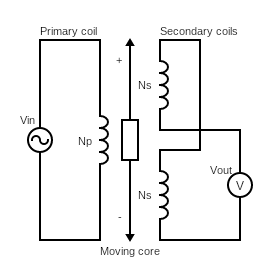
\includegraphics[width=0.4\textwidth]{sensor-theory/displacement-lvdt}
  \caption{\label{img:lvdt}Schemat układu przetwornika LVDT}
\end{figure}

Uzwojenie pierwotne zasilane jest napięciem przemiennym.~W~uzwojeniach wtórych (oznaczone jako Ns na
schemacie) indukują się napięcia, które zależne są od położenia rdzenia wewnątrz obudowy. Gdy rdzeń
znajduje się~w~równej odległości od obu cewek wtórnych -- napięcia będą sobie równe. Ponieważ układ
sensora LVDT jest zbudowany na podstawie transformatora różnicowego, to napięcie na wyjściu całego
układu będzie równe różnicy napięć na cewkach wtórnych. Zależność tę opisuje wzór
\cite{sensory_wykład}:

\begin{equation}
  u_{wy}=u_1-u_2=U_1 \sin{(\omega t + \varphi_1)} - U_2 \sin{(\omega t + \varphi_2)}
\end{equation}

Natomiast charakterystykę przetwarzania przetwonika LVDT (zależność napięcia wyjściowego oraz
przesunięcia rdzenia względem punktu równowagi) opisuje się wzorem:

\begin{equation}\label{eqn:theory-lvdt}
  U_{wy}=f\cdot I_p\cdot\bigg(4\pi\cdot N_p N_w\cdot \mu_0\cdot l_p\cdot\frac{x}{3l_w}\cdot
  \log{\Big(\frac{r_o}{r_i}\Big)}\bigg)\bigg(1-\frac{x^2}{2l_p^2}\bigg)
\end{equation}

\begin{eqparams}
  f & częstotliwość zasilania układu,\\
  I_p & prąd~w~uzwojeniu pierwotnym $I_p=\cfrac{U_{wej}}{R}$,\\
  N_p,\,N_w & liczba zwojów~w~uzwojeniach, odpowiednio~w~pierwotnym~i~wtórnych,\\
  l_p,\,l_w & długości uzwojeń, odpowiednio pierwotnego~i~wtórnych,\\
  \mu_0 & przenikalność magnetyczna próżni ($4\pi\cdot 10^{-7}$),\\
  x & przesunięcie rdzenia względem stanu ustalonego,\\
  \cfrac{r_o}{r_i} & stosunek promieni zewnętrzynych~i~wewnętrznych układu cewki,\\
\end{eqparams}

Charakterystyka przetwarzania sensora, przedstawiona na rysunku \ref{img:transfer-lvdt}, ma kształt
litery ,,V'', obie strony są symetryczne względem punktu zerowego -- stanu zrównoważenia. Dodatkowo,
napięcie wyjściowe nie jest zerowe~w~stanie równowagi -- jest to spowodowane niewielkimi różnicami
pomiędzy uzwojeniami wtórnymi \cite{sensory_wykład}.

\addimage{0.9}{sensor-theory/transfer-lvdt}{\label{img:transfer-lvdt}Przykładowa charakterystyka
  przetwarzania sensora LVDT~w~zależności od przesunięcia}

Sensory LVDT najczęściej stosuje się~w~zakresie $\pm$5 do $\pm$250mm, przy czym możliwe jest
mierzenie większych zakresach, jednakże wiąże się to ze znacznym zwiększeniem rozmiarów samego
przetwornika. Wykorzystanie przetwornika fazoczułego przy pomiarach przetwornikiem
LVDT pozwala na używanie jego pełnego zakresu, ponieważ możliwe jest określenie po której
stronie względem punktu równowagi znajduje się rdzeń. Napięcie wyjściowe z układu określa się wtedy
równianiem:

\begin{equation}
  U_{wy}=k\cdot{U_{wej}}\cdot\cos{(\varphi)}
\end{equation}

\begin{eqparams}
  k & współczynnik proporcjonalności,\\
  U_{wej} & napięcie wejściowe,\\
  \varphi & przesunięcie fazowe.
\end{eqparams}

Jeżeli napięcie wejściowe oraz wyjściowe będą w fazie, to kąt przesunięcia fazowego będzie
równy~0$^\circ$. Cosinus będzie wtedy równy 1. Natomiast w przeciwnej sytuacji (sygnały w
przeciwfazie), kąt $\varphi$ będzie równy 180$^\circ$, a cosinus będzie równy -1. Stosując
przetwornik fazoczuły przedstawiona powyżej charakterystyka przetwornika przyjmie postać
przedstawioną na rysunku \ref{img:transfer-lvdt-full}.

\addimage{0.9}{sensor-theory/transfer-lvdt-full}{\label{img:transfer-lvdt-full}Charakterystyka
  przetwarzania sensora LVDT po zastosowaniu przetwornika fazoczułego}

Sensory można stosować~w~dwóch typach układu: AC/AC oraz DC/DC.~W~przypadku układów
napięcia przemiennego otrzymuje się teoretycznie nieskończoną rozdzielczość pomiarową, większą
wytrzymałość mechaniczną przetwonika oraz mniejsze rozmiary układu. Natomiast korzystając~z~układów
napięcia stałego nie jest wymagane korzystanie~z~układów kondycjonujących sygnał oraz kompensujących
błędy pomiarowe. Częściej stosowane są jednak układy AC/AC~z~uwagi na zalety przeważające nad
układami DC/DC.


% Sensory naprężenia - Strain gauge
\section{Sensory naprężenia}
Czujniki naprężenia operują w oparciu o zjawisko zmiany rezystancji materiału, z którego sensor
jest wykonany, pod wpływem naprężeń mechanicznych. Zmiana rezystancji spowodowana jest odkształcaniem
się elementu, do którego przytwierdzony jest przetwornik tensometryczny. Podstawową funkcję
przetwarzania tensometrów opisuje równanie \cite{hoffman1989, milek2006}:

\begin{equation}
  \frac{dR}{R}=\varepsilon\cdot(1+2\nu)+\frac{d\varrho}{\varrho}
\end{equation}

\begin{eqparams}
  R & rezystancja początkowa tensometru, \\
  \varepsilon & wartość odkształcenia, definiowana jako $\varepsilon=\cfrac{dl}{l}$, \\
  \nu & współczynnik Poissona, \\
  \varrho & rezystywność materiału tensometru (rezystora)
\end{eqparams}

\subsection{Tensometry}
Na zmianę parametrów czujnika tensometrycznego metalowego największy wpływ ma wartość odkszałcenia
elementu, na którym zamontowany jest sensor. Jednakże istotną rolę dla pracy przetwornika stanowi
wpływ temperatury otoczenia. Negatywny wpływ temperatury można skompensować poprzez odpowiedni dobór
parametrów tensometru na etapie produkcji -- dodając do podstawowego materiału sensora odpowiednie
domieszki. Przetworniki tensometryczne przetwarzają nieelektryczną wielkość odkształcenia
$\varepsilon$ na wielkość elektryczną -- zmianę rezystancji. Następnie~w~torze pomiarowym stosuje
się przetwornik pozwalający na generowanie mierzalnego sygnału napięciowego.

Jeżeli element, na którym zamontowane są tensometry ulegnie odkształceniu, to zmieni się wartość
rezystancji sensora. Wartości zmian rezystancji mogą być dodatnie lub ujemne, jest to zależne od
kierunku~w~jakim odkształca się czujnik. Przedstawia to wzór \cite{gawedzki2010}:

\begin{equation}
  R_i = R_{i\,0} \pm \Delta R_i, \quad\quad\quad \text{gdzie:}\quad i=1,2,3,4
\end{equation}

Zmianę wartości rezystancji przetwornika tensometrycznego przedstawia zależność opisana wzorem
\ref{eqn:strain-r}, natomiast~w~przypadku, gdy brany jest pod uwagę wpływ temperatury zależność ta
przedstawiona jest wzorem \ref{eqn:strain-temp}.

\begin{equation}\label{eqn:strain-r}
  \Delta R_i = R_i\cdot\varepsilon\cdot k
\end{equation}

\begin{equation}\label{eqn:strain-temp}
  \Delta R_i = R_i(\varepsilon\cdot k + \alpha\Delta T)
\end{equation}

\begin{eqparams}
  R_i & bazowa rezystancja tensometru,\\
  \varepsilon & wartość odkształcenia,\\
  k & współczynnik odkształcenia (stała tensometryczna)\\
  \alpha & współczynnik temperaturowy metalu (zgodnie~z~tabelą \ref{tab:temp_alpha}),\\
  \Delta T & różnica temperatur pomiędzy temperaturą otoczenia~a~odniesienia (20\degC),\\
\end{eqparams}

Do pomiarów tensometrycznych często stosuje się układy mostkowe. Zastowanie takiego układu pozwala
eliminację składowej siły powodującej odkształcenie, która nie jest mierzona. Dodatkowo dzięki
zastosowaniu mostka możliwa jest kompensacja zakłóceń związanych ze zmianami temperatury otoczenia
podczas pomiaru.

Wyróżnia się trzy konfiguracje mostka tensometrycznego:
\begin{itemize}
  \item [--] układ ćwierćmostkowy~z~jednym pracującym tensometrem
  \item [--] układ półmostkowy~z~dwoma czynnymi tensometrami (występują dwa rodzaje tej
        konfiguracji,~z~tensometrami~w~ramionach sąsiednich lub przeciwległych),
  \item [--] układ pełnomostkowy~z~czterema aktywnymi tensometrami.
\end{itemize}
Wszystkie układy mają różną skuteczność kompensacji wpływu temperatury. Na
rysunku~\ref{img:strain-gauge} przedstawiony został schemat układu mostkowego.

\addimage{0.65}{sensor-theory/strain-gauge}{\label{img:strain-gauge}Schemat układu mostkowego}

\paragraph{Układ ćwierćmostkowy:} Posiada jeden czynny tensometr (przykładowo~w~pierwszym ramieniu
mostka), do wyznaczenia napięcia na wyjściu układu, korzystając~z~zależności \ref{eqn:strain-temp},
stosuje się równanie:

\begin{equation}
  U_{wy}=\cfrac{1}{4}\cdot{U_z}\cdot\cfrac{\Delta R_1}{R_1}=\cfrac{1}{4}\cdot{U_z}\cdot({k}
  \cdot\varepsilon_1+{k_1}\cdot\alpha_1\Delta{T_1})
\end{equation}

Na podstawie tego równania można stwierdzić, że układ nie będzie kompensował wpływu temperatury.

\paragraph{Układ półmostkowy:} Posiada dwa czynne tensometry. Jeżeli zastostuje się
wariant~z~tensometrami~w~sąsiednich ramionach (przykładowo pierwszym~i~trzecim), to napięcie
wyjściowe wyznacza się~z~zależności:

\begin{equation}\label{eqn:half-bridge-adj}
  U_{wy}=\cfrac{1}{4}\cdot{U_z}\cdot\bigg(\cfrac{\Delta R_1}{R_1}-\cfrac{\Delta R_3}{R_3}\bigg)=
  \cfrac{1}{4}\cdot{U_z}\cdot\big({k}\cdot(\varepsilon_1-\varepsilon_3)+{k_1}\cdot(\alpha_1
  \Delta{T_1}-\alpha_3\Delta{T_3})\big)
\end{equation}

Jeżeli obecne~w~układzie tensometry będą pracować~w~takiej samej temperaturze, to wpływ temperatury
zostanie skompensowany~i~napięcie wyjściowe będzie można wyznaczyć korzystając~z~równania:

\begin{equation}\label{eqn:half-bridge-compensation}
  U_{wy}=\cfrac{1}{4}\cdot{U_z}\cdot\big({k}\cdot(\varepsilon_1-\varepsilon_3)\big)
\end{equation}

Natomiast~w~przypadku zastosowania wariantu~o~ramionach przeciwległych (przykładowo~z~tensometrami
włączonymi do ramion pierwszego~i~czwartego) to zależność \ref{eqn:half-bridge-adj} przyjmie postać:

\begin{equation}
  U_{wy}=\cfrac{1}{4}\cdot{U_z}\cdot\bigg(\cfrac{\Delta R_1}{R_1}-\cfrac{\Delta R_3}{R_3}\bigg)=
  \cfrac{1}{4}\cdot{U_z}\cdot\big({k}\cdot(\varepsilon_1+\varepsilon_3)+{k_1}\cdot(\alpha_1
  \Delta{T_1}+\alpha_3\Delta{T_3})\big)
\end{equation}
~i~nie nastąpi kompensacja, natomiast wynik pomiaru będzie zawierał błąd związany~z~negatywnym
wpływem temperatury.

\paragraph{Układ pełnomostkowy:} Posiada cztery tensometry włączone do każdego~z~ramion mostka.
Napięcie wyjściowe wyznacza się równaniem:

\begin{align}
  U_{wy} & =\cfrac{1}{4}\cdot{U_z}\cdot\bigg(\cfrac{\Delta R_1}{R_1}+\cfrac{\Delta R_2}{R_2}-
  \cfrac{\Delta R_3}{R_3}+\cfrac{\Delta R_4}{R_4}\bigg)=              \nonumber               \\
         & =\cfrac{1}{4}\cdot{U_z}\cdot\big({k}\cdot
  (\varepsilon_1+\varepsilon_2-\varepsilon_3+\varepsilon_4)+{k_1}\cdot(\alpha_1\Delta{T_1}+
  \alpha_2\Delta{T_2}-\alpha_3\Delta{T_3}+\alpha_4\Delta{T_4})\big)
\end{align}

Zakładając identyczne warunki termiczne~w~otoczeniu każdego sensora można stwierdzić, że wpływ
temperatury zostanie skompensowany.~W~takim przypadku napięcie wyjściowe będzie można wyznaczyć
korzystając~z~równania \ref{eqn:half-bridge-compensation} uzupełnionego~o~dwa dodatkowe
tensometry~w~układzie:

\begin{equation}
  U_{wy}=\cfrac{1}{4}\cdot{U_z}\cdot\big({k}\cdot(\varepsilon_1+\varepsilon_2-\varepsilon_3+
  \varepsilon_4)\big)
\end{equation}

\begin{eqparams}[W każdym~z~powyższych wzorów (przyjmując \textit{\textrm{i}} = 1,2,3,4):]
  \Delta R_i & zmiana rezystancji i-tego tensometru (wartość może być dodatnia lub ujemna)\\
  R_i & bazowa rezystancja i-tego tensometru\\
  k & współczynnik odkształceń (stała tensometryczna)\\
  \varepsilon_i & odkształcenie i-tego tensometru\\
  U_z & napięcie zasilania układu mostkowego\\
  \alpha_i & współczynnik temperaturowy materiału i-tego tensometru\\
  \Delta{T_i} & różnica temperatur pomiędzy temperaturą otoczenia~a~odniesienia (20\degC)\\
\end{eqparams}

We wzorach pojawia się dodatkowa stała $k_1$, ponieważ rzeczywiste stałe tensometryczne
odbiegają od wartości założonych przez producenta sensora~w~fazie projektowania.

Problem braku kompensacji temperaturowej~w~układach ćwierćmostkowym oraz półmostkowym~z~ramionami
przeciwległymi można rozwiązać poprzez zastosowanie tensometrów biernych. Montuje się je~w~pobliżu
dwóch czynnych tensometrów, jednakże bez przytwierdzania ich do elementu, którego odkształcenia są
mierzone \cite{gawedzki2010}.~W~takiej konfiguracji sensory bierne nie zmieniają swojej rezystancji
na skutek działającej siły,~a~tylko przez zmianę temperatury, dzięki czemu umożliwią kompensowanie
jej wpływu.


